\section{What version 1 taught us}\label{sec:audit}

The v1 note defined a forest vulnerability score, $\mathrm{FVS}=\int(\alpha\,\Delta\VPD+\beta\,\Delta T_{\max}-\gamma\,\Delta P)\,\sigma(H)^{-1}\,dt$, with $\alpha,\beta,\gamma$ to be read off random-forest importances, and the repository trained a random forest to predict $\sigma(H)$, the local standard deviation of canopy height, from three growing-season climate deltas on 4\,338 one-kilometre pixels. A Streamlit app then added scenario deltas to the table and reported the shortfall of predicted against observed $\sigma(H)$ as vulnerability. It is a working end-to-end prototype, which is exactly why we can be specific about what has to change. We re-ran the delivered table and model (\texttt{scripts/audit\_v1.py}; the hyper-parameters, seed and split reproduce the published $R^2=0.292$ and MAE $=1.80$~m exactly), and Table~\ref{tab:audit} lists what we found.

\begin{table}[t]
\centering
\caption{Audit of the v1 training table and model. All numbers are recomputed from \texttt{Armenia\_ML\_Training\_Data.parquet} ($n=4\,338$ pixels; RF: 500 trees, depth 15, seed 42).}\label{tab:audit}
\footnotesize
\renewcommand{\arraystretch}{1.1}
\begin{tabularx}{\linewidth}{@{}>{\raggedright\arraybackslash\bfseries\sffamily}p{2.55cm}>{\raggedright\arraybackslash}X>{\raggedright\arraybackslash}p{4.6cm}@{}}
\toprule
Finding & Evidence & Consequence for v2\\
\midrule
Validation leaks space & Random 80/20 split: $R^2=0.29$, MAE 1.80~m (predicting the mean: 2.13~m). Blocked 5-fold CV: $R^2=0.20,\,0.11,\,0.04,\,-0.28,\,-0.45$ for 5, 10, 25, 50, 75~km blocks. Median nearest-neighbour spacing 0.7~km; neighbours correlate at $r=0.97$--$0.997$ in every feature and 0.58 in the target. & Skill was interpolation between near-duplicates. Block size must come from the data and the CV must mimic the use (\S\ref{sec:ml}).\\
The features are coordinates & The three deltas predict longitude and latitude with $R^2=0.87$ and $0.89$. Longitude and latitude alone reach $R^2=0.45$ on the same random split, and $-0.06$ at 25~km blocks against 0.04 for the climate features. & A climate model must beat a coordinates-only baseline under blocked CV, or it has learned nothing about climate.\\
Extrapolation is a constant & Training range of $\Delta T_{\max}$ is 0.05--0.10~K. Adding any warming $\ge 0.25$~K changes no prediction (max difference $4\times10^{-16}$~m). Mean FVS is 60.6\,\% for SSP1-2.6 mid-century and 64.6\,\% for SSP5-8.5 end-century, against 6.6\,\% with deltas as observed: the mildest scenario already produces 54 of the 58 points by which the harshest exceeds the no-forcing baseline (Fig.~\ref{fig:v1}b). & Outside the training support the model must hand over to physics, and say so (\S\ref{sec:gate}).\\
The label measures structure & $\sigma(H)$ is predicted from mean height alone with $R^2=0.67$; its median coefficient of variation is 0.58. At 1~km it mostly reflects cover fraction and stand mosaic, not physiological stress. & The response must be an event that happened to a tree or stand (dieback, growth collapse, planting failure).\\
Importances are not coefficients & Gini importances are 34.9, 31.4 and 33.7\,\% for VPD, $T_{\max}$ and $P$: near-equal, unsigned, and taken from a model that cannot extrapolate. They were described as SHAP values and proposed as $\alpha,\beta,\gamma$. & Effects come from a hazard model with signs and units; ALE and SHAP are used to explain, never to parametrise.\\
Units and construction & $\Delta\VPD/\Delta T_{\max}=0.83$~kPa~K$^{-1}$ in the table; at fixed relative humidity it should be 0.03--0.25. Training VPD (CHELSA) and scenario VPD (CMIP6-derived) are built differently, and the deltas themselves are small (mean $\Delta T_{\max}=0.07$~K). & One VPD construction end to end, checked by a thermodynamic unit test (\S\ref{sec:A}).\\
No time, no events, survivors only & One row per pixel; no year, no exposure, no mortality event. The forest mask conditions on persistence, so pixels that died are excluded by construction. & Event histories for every pixel that was forest at the start, with harvest and fire as competing events (\S\ref{sec:C}).\\
Score $\neq$ formula & The app evaluates $\mathrm{clip}\big((\sigma_{\text{obs}}-\sigma_{\text{pred}})/\sigma_{\text{obs}}\times100,0,100\big)$, a model residual, not the time integral of the concept note. & Estimand defined once, in probability units (\S\ref{sec:estimand}).\\
\bottomrule
\end{tabularx}
\end{table}

\begin{figure}[t]
\centering
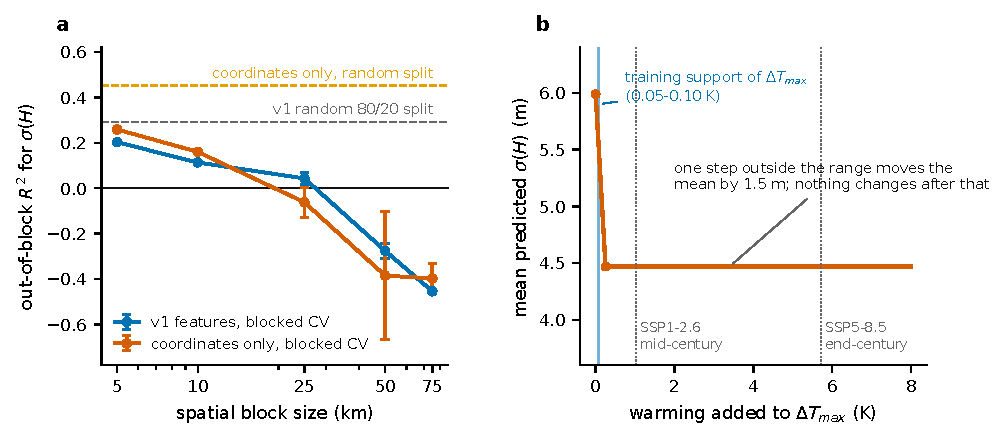
\includegraphics[width=\linewidth]{fig1_v1_audit.pdf}
\caption{The v1 model, audited on its own data. (a) Out-of-block $R^2$ against block size for the v1 features (blue) and for coordinates alone (vermilion); dashed lines show the random-split scores. Points are means of three block assignments, bars $\pm$1~SD. (b) Mean predicted $\sigma(H)$ as extra warming is added to $\Delta T_{\max}$ with the other two deltas unchanged: one step outside the training range moves the mean by 1.5~m and nothing moves it afterwards.}\label{fig:v1}
\end{figure}

None of this diminishes what v1 achieved. It settled the data plumbing, the raster conventions, and a demonstrable interface, and it made the central problem legible: when a model is trained on the spatial pattern of a static quantity, it learns geography, and geography does not project. Everything that follows is designed to make that failure impossible to repeat, and to replace a single number with a chain of quantities that can each be checked against something observable.
